\chapter{Experimento}
\label{cap:experimento}
O presente trabalho apresentou um processo de alinhamento de dados independente de contexto. Esse processo foi consolidado em uma ferramenta para realizar a correspondência de instâncias. Este capítulo apresenta o experimento realizado para análise da eficácia do alinhamento de dados à partir do processo e ferramenta propostos. O capítulo está dividido em quatro seções que abordam (i) \textit{Design} de experimento; (ii) Execução do experimento; (iii) Análise dos resultados e (iv) Principais conclusões obtidas.

\section{Configuração de Experimento}
Nesta seção, será detalhado o planejamento do experimento que foi projetado para este trabalho. Dentro do planejamento, encontra-se a definição da questão de pesquisa e derivação de hipóteses, a seleção das variáveis dependentes e independentes, a identificação da unidade experimental e a seleção do modelo experimental que será utilizado.

\subsection{Situando o problema}
A avaliação de ferramentas de correspondência de instâncias utiliza dois \textit{datasets} e um alinhamento de referência. Como mencionado na subseção \ref{contribuicao}, isso permite que os desenvolvedores utilizem computação específica para os \textit{datasets}. Com isso, retomamos o nosso problema:

\textbf{(Problema Geral)} Como identificar que duas instâncias referem-se à mesma entidade do mundo real?
Atualmente, estratégias baseadas em similaridade, aprendizagem, regras e contexto \cite{castano2011ontology} vêm sendo utilizadas para resolver o problema. Porém, segundo \citeonline{homoceanu2014putting} essa ferramentas para correspondência de instância não estão prontas para alinhar dados automaticamente de forma confiável. 

Diante disso, nos deparamos com nosso problema específico: 

\textbf{(Problema Específico)} Como melhorar a eficácia das ferramentas para correspondência de instâncias?

\subsection{Objetivos da Investigação}
A pesquisa a ser realizada é de caráter experimental e tem como objetivo geral \textbf{avaliar a eficácia das ferramentas de correspondência de instâncias}. O intuito do experimento é \textbf{refutar} as hipóteses nulas definidas na subseção \ref{sub:hipoteses}, indicando que a abordagem proposta, apesar de não conter computação específica para os \textit{datasets}, é capaz de criar correspondências com eficácia.

Formalmente, o objetivo da nossa investigação pode ser definido como analisar ferramentas de correspondência de instâncias com a intenção de compará-las a respeito de sua eficácia no ponto de vista de geração de correspondência entre instâncias, no contexto de alinhamento de dados entre \textit{datasets}, com o fim de utilizar as melhores abordagens provendo uma melhoria na qualidade das ferramentas.

Como objetivos específicos, temos:
\begin{enumerate}
	\item[i)] Comparar a abordagem proposta e as existentes;
	\item[ii)] Avaliar empiricamente a qualidade dos modelo criado.
\end{enumerate}


\subsection{Questões de Pesquisa e Hipóteses}
\label{sub:hipoteses}
Após a apresentação dos objetivos deste experimento, nos deparamos com a seguinte questão de pesquisa e suas respectivas hipóteses:

%\textbf{Q1} Existe diferença na eficácia entre AML, RiMOM-2016 e a solução proposta? Se sim, qual abordagem foi melhor?
\textbf{Q1} Como se comportam as ferramentas para correspondência de instâncias (AML, RiMOM-2016 e Proposta) com relação a eficácia? 

A questão de pesquisa acima implica nas seguintes hipóteses de pesquisa:

\begin{itemize}
\item H1-0: A precisão apresentada pelas abordagens é igual.
\item H1-1: A precisão apresentada pelas abordagens é diferente.
\item H2-0: A revocação apresentada pelas abordagens é igual.
\item H2-1: A revocação apresentada pelas abordagens é diferente.
\item H3-0: A medida-f apresentada pelas abordagens é igual.
\item H3-1: A medida-f apresentada pelas abordagens é diferente.
\end{itemize}

\subsection{Fatores e Variáveis de Resposta}
A partir da definição das hipóteses na subseção \ref{sub:hipoteses}, temos os fatores, também conhecidos como variáveis independentes, como sendo:
\begin{itemize}
	\item \textbf{Ferramenta:} Esta variável especifica qual a ferramenta de alinhamento será avaliada
\end{itemize}

Como variáveis de resposta, também conhecidas como variáveis dependentes, nós temos:

\textbf{Precisão (P):} Para a correspondência de instâncias, indica a quantidade de correspondências que são relevantes em relação a todas as correspondências geradas pelas ferramentas. A definição formal para esta métrica é descrita pela equação abaixo:

\begin{equation}
P = \dfrac{|{A}\cap{B}|}{|A|}
\end{equation}

\textbf{Revocação (R):} Para a correspondência de instâncias, indica a quantidade de correspondências relevantes com relação ao conjunto de todas as correspondências possíveis (espelho). A definição formal para esta métrica é descrita pela equação abaixo:

\begin{equation}
R = \dfrac{|{A}\cap{B}|}{|B|}
\end{equation}

\textbf{Medida-f (F):} Média harmônica entre precisão e revocação. A intenção é transformar essas duas métricas em apenas uma. A definição formal para esta métrica é descrita pela equação abaixo:

\begin{equation}
F = \dfrac{{2}\cdot{P}\cdot{R}}{P+R}
\end{equation}

\subsection{Níveis dos Fatores}
\label{sub:fator_nivel}
Os níveis dos fatores são apresentados na Tabela \ref{tab:factor_levels}.

\begin{table}[h]
	\centering
	\caption{Níveis de fatores}
	\label{tab:factor_levels}
	\begin{tabular}{|c|c|c|}
		\hline
		\textbf{Fator}        & \textbf{Nível} &  \textbf{Descrição}   \\ \hline
		\multirow{3}{*}{Ferramenta} &       F1       &    Ferramenta AML     \\ \cline{2-3}
		&       F2       & Ferramenta RiMOM-2016 \\ \cline{2-3}
		&       F3       &       Proposta       \\ \hline
	\end{tabular}
\end{table}

\subsection{Definição formal das Hipóteses}
% * <profsean@gmail.com> 2017-01-19T01:59:54.731Z:
% 
% > Definição formal das Hipóteses
% Para mim não é isto... Você não quer saber se são iguais ou diferentes, mas se a proposta consegue um alinhamento melhor (e em quais condições)... Deste modo, seria uma questão de verificar se a diferença de valores é estatisticamente significativa (o que não me parece ser) e porque o desempenho da proposta foi melhor no cenário 1 e intermediário no cenário 2...
% 
% ^ <armandobs14@gmail.com> 2017-01-19T18:15:23.403Z:
% 
% Foi utilizado o teste de fisher para verificar a validação de hipóteses.
% 
% ^ <armandobs14@gmail.com> 2017-01-20T05:11:17.970Z.
Formalmente, todas as hipóteses definidas na seção \ref{sub:hipoteses} podem ser definidas conforme a Tabela \ref{tab:hypothesis}. P, R e F são funções que retornam, respectivamente a precisão, revocação e medida-f, com relação às abordagens F1 (AML), F2 (RiMOM-2016) e F3 (Proposta).

\begin{table}[h]
	\centering
	\caption{Formalização das hipóteses}
	\label{tab:hypothesis}
	\begin{tabular}{|c|c|c|}
		\hline
		Hipótese &                      Hipótese Nula                      &                        Hipótese Alternativa                         \\ \hline
		   H1    & H1-0:$ P(F_i) = P(F_j); i,j \in \{1,2,3\}; i \not= j  $ & H1-1:$ \exists i,j \in \{1,2,3\}; i \not= j ; P(F_i) \not= P(F_j) $ \\ \hline
		   H2    & H2-0:$ R(F_i) = R(F_j); i,j \in \{1,2,3\}; i \not= j  $ & H2-1:$ \exists i,j \in \{1,2,3\}; i \not= j ; R(F_i) \not= R(F_j) $ \\ \hline
		   H3    & H3-0:$ F(F_i) = F(F_j); i,j \in \{1,2,3\}; i \not= j  $ & H3-1:$ \exists i,j \in \{1,2,3\}; i \not= j ; F(F_i) \not= F(F_j) $ \\ \hline
	\end{tabular}
\end{table}

\subsection{Unidades Experimentais}
Levando em consideração as diversas classificações de experimento \cite{montgomery2012design}, o presente experimento é classificado como fatorial completo com blocagem. A blocagem foi escolhida com o objetivo de suprimir os efeitos dos \textit{datasets} nas variáveis resposta. Para cada cenário houve a execução de todos os níveis de fatores, garantindo a completude do experimento.

\subsection{Plano de execução}
A Figura \ref{fig:experiment} apresenta os passos de execução de cada alinhamento, que são descritos abaixo:
\begin{itemize}
	\item Construir contêiner com as configurações zeradas;
	\item Carregar dos dados;
	\item Executar ferramenta dentro do contêiner;
	\item Coletar dados de alinhamento;
	\item Destruir contêiner;
	\item Analisar dados.
\end{itemize}

\begin{figure}[h]
	\centering
	\includegraphics[width=0.9\textwidth]{./imagens/experimento.pdf}
	\caption{Processo de execução do experimento}
	\label{fig:experiment}
\end{figure}

\subsection{Coleta dos Dados}
Os dados utilizados neste estudo foram fornecidos pela OAEI. O \textit{dataset}\footnote{\url{http://islab.di.unimi.it/content/im_oaei/2016/\#doremus}} é composto por três variações (\textit{9-heterogeneities}, \textit{4-heterogeneities} e \textit{falsepositives-trap}). Cada uma das variações conta com um alinhamento de referência, para que seja possível calcular as métricas.

%-----------------------------------------------------------
\section{Execução do experimento}
Para avaliar as ferramentas para correspondência de instância, o experimento irá contar com dois cenários possíveis, com uma execução para cada nível dos fatores definidos na subseção \ref{sub:fator_nivel}, totalizando 6 execuções. A Tabela \ref{tab:cenarios} apresenta os cenários. 

\begin{table}[h]
	\centering
	\caption{Cenários de alinhamento}
	\label{tab:cenarios}
	\begin{tabular}{|c|c|}
		\hline
		\textbf{Cenário} & \textbf{Datasets}          \\ \hline
		C1               & 9-heterogeneities          \\ \hline
		C2               & falsepositives-trap        \\ \hline
	\end{tabular}
\end{table}

\subsection{Instrumentação}
Para a realização do experimento de correspondência de instâncias, serão utilizados os seguintes instrumentos.

\begin{itemize}
\item Intellij IDEA 2016.3 para desenvolvimento do código e execução da proposta.
\item Virtuoso RDF Store - 07.20.3217;
\item OpenJDK 64-Bit Server VM (build 25.111-b14, mixed mode)
\end{itemize}

Para isolar os efeitos entre as execuções, todo o experimento foi conduzido em um contêiner, que permite isolar as aplicações, fazendo com que as aplicações sejam executadas em ambientes idênticos sem que gerem efeitos colaterais entre si.

\subsection{Ameaças à validade}
Embora todo experimento tenha sido projetado para minimizar possíveis ameaças que comprometam suas conclusões, existem algumas ameaças que devem ser mencionadas. Nos tópicos a seguir, serão apresentadas e detalhadas as ameaças deste experimento.
\begin{itemize}
\item \textbf{Ameaças à validade interna:}\\
Uma possível ameaça interna à validade do experimento pode ser a seleção das unidades experimentais, pois os \textit{dataset} utilizados no experimento foram fornecidos pelo OAEI e nenhum outro \textit{dataset} foi utilizado.

\item \textbf{Ameaças à validade externa}\\
As unidades experimentais desta pesquisa são selecionadas de apenas uma base de dados correspondente a cada modelo, tendo, cada uma delas, características que poderão não ser generalizadas para as demais bases

\item \textbf{Ameaças à validade de construto}\\
É possível que a quantidade de fatores e cenários não sejam suficientes para observar diferenças significativas na eficácia entre as abordagens utilizadas para a correspondência de instâncias. Além disso, deve-se considerar que o tempo de resposta não foi considerado no experimento.

\item \textbf{Ameaças à validade de conclusão}\\
Devido à pequena quantidade de dados por \textit{dataset}, é possível que a quantidade de instâncias por \textit{dataset}, não seja suficiente para observar diferenças significativas nas métricas associadas.

\end{itemize}

\section{Análise dos Resultados}
O experimento foi conduzido de acordo com o planejamento descrito anteriormente neste capítulo. Depois da execução, os \textit{datasets} de alinhamento foram coletados. Os dados de precisão, revocação e medida-f foram calculados de acordo com as funções especificadas anteriormente. Ao longo desta seção, uma análise descritiva dos dados obtidos será apresentada com as métricas referentes a cada cenário.

As figuras \ref{fig:cenario1} e \ref{fig:cenario2} apresentam as ferramentas de acordo com seus resultados em cada um dos cenários. A Tabela \ref{tab:resultados} sumariza os dados obtidos para cada cenário.

\begin{table}[h]
	\centering
	\caption{Sumarização dos dados relativos a precisão, revocação e medida-f por cenário.}
	\label{tab:resultados}
	\begin{tabular}{|c|c|c|c|c|}
		\hline
		      Cenário       & Ferramenta & Precisão & Revocação & Medida-F \\ \hline
		\multirow{3}{*}{C1} &  Proposta  &    1     &   0.875   &  0.933   \\ \cline{2-5}
		                    &    AML     &  0.966   &   0.875   &  0.918   \\ \cline{2-5}
		                    &   RiMOM    &  0.813   &   0.813   &  0.813   \\ \hline
		\multirow{3}{*}{C2} &    AML     &  0.921   &   0.854   &  0.886   \\ \cline{2-5}
		                    &  Proposta  &  0.906   &   0.707   &  0.794   \\ \cline{2-5}
		                    &   RiMOM    &  0.707   &   0.707   &  0.707   \\ \hline
	\end{tabular}
\end{table}

\begin{center}
\begin{figure}
	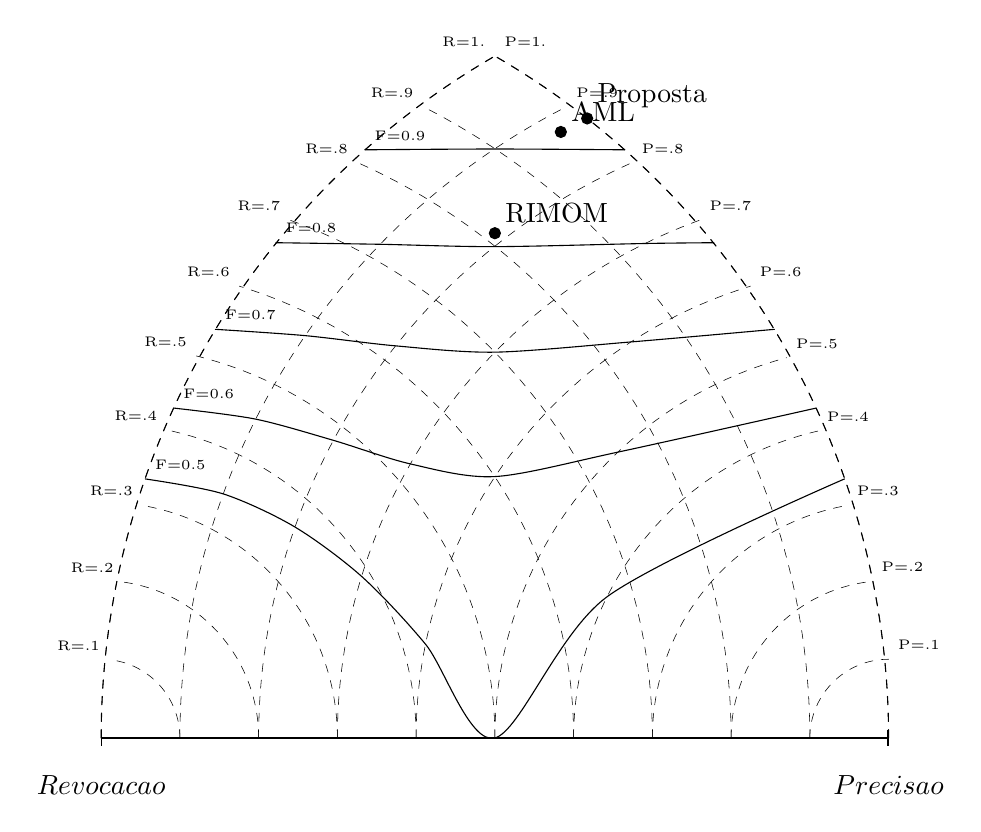
\begin{tikzpicture}[cap=round]{H}
	%\draw[step=1cm,very thin,color=gray] (0,0) grid (10.0,9.0);
	\draw[|-|] (-0,0) -- (10,0);
	\draw[dashed,very thin] (10,0) arc (0:60:10cm);
	\draw[dashed,very thin] (0,0) arc (180:120:10cm);
	\draw[dashed] (10,0) arc (0:60:10cm) node[anchor=south east]  {{\tiny R=1.}};
	\draw[dashed,very thin] (9,0) arc (0:63:9cm) node[anchor=south east] {{\tiny R=.9}};
	\draw[dashed,very thin] (8,0) arc (0:66:8cm) node[anchor=south east]  {{\tiny R=.8}};
	\draw[dashed,very thin] (7,0) arc (0:70:7cm) node[anchor=south east]  {{\tiny R=.7}};
	\draw[dashed,very thin] (6,0) arc (0:73:6cm) node[anchor=south east]  {{\tiny R=.6}};
	\draw[dashed,very thin] (5,0) arc (0:76:5cm) node[anchor=south east] {{\tiny R=.5}};
	\draw[dashed,very thin] (4,0) arc (0:78:4cm) node[anchor=south east] {{\tiny R=.4}};
	\draw[dashed,very thin] (3,0) arc (0:80:3cm) node[anchor=south east] {{\tiny R=.3}};
	\draw[dashed,very thin] (2,0) arc (0:82:2cm) node[anchor=south east] {{\tiny R=.2}};
	\draw[dashed,very thin] (1,0) arc (0:84:1cm) node[anchor=south east] {{\tiny R=.1}};
	\draw[dashed] (0,0) arc (180:120:10cm) node[anchor=south west] {{\tiny P=1.}};
	\draw[dashed,very thin] (1,0) arc (180:117:9cm) node[anchor=south west] {{\tiny P=.9}};
	\draw[dashed,very thin] (2,0) arc (180:114:8cm) node[anchor=south west] {{\tiny P=.8}};
	\draw[dashed,very thin] (3,0) arc (180:110:7cm) node[anchor=south west] {{\tiny P=.7}};
	\draw[dashed,very thin] (4,0) arc (180:107:6cm) node[anchor=south west] {{\tiny P=.6}};
	\draw[dashed,very thin] (5,0) arc (180:105:5cm) node[anchor=south west] {{\tiny P=.5}};
	\draw[dashed,very thin] (6,0) arc (180:103:4cm) node[anchor=south west] {{\tiny P=.4}};
	\draw[dashed,very thin] (7,0) arc (180:100:3cm) node[anchor=south west] {{\tiny P=.3}};
	\draw[dashed,very thin] (8,0) arc (180:96:2cm) node[anchor=south west] {{\tiny P=.2}};
	\draw[dashed,very thin] (9,0) arc (180:90:1cm) node[anchor=south west] {{\tiny P=.1}};
	\draw (0.56,3.29) node[anchor=south west] {\tiny{F=0.5}};
	\draw plot[smooth] coordinates { (0.56,3.29) (1.55,3.10) (2.46,2.68) (3.31,2.05) (4.12,1.19) (5.00,0.00) (6.42,1.79) (9.44,3.29)};
	\draw (0.92,4.19) node[anchor=south west] {\tiny{F=0.6}};
	\draw plot[smooth] coordinates { (0.92,4.19) (1.96,4.05) (2.95,3.78) (3.93,3.48) (5.00,3.32) (6.56,3.63) (9.08,4.19)};
	\draw (1.45,5.19) node[anchor=south west] {\tiny{F=0.7}};
	\draw plot[smooth] coordinates { (1.45,5.19) (2.59,5.11) (3.74,4.98) (5.00,4.90) (6.73,5.03) (8.55,5.19)};
	\draw (2.22,6.29) node[anchor=south west] {\tiny{F=0.8}};
	\draw plot[smooth] coordinates { (2.22,6.29) (3.54,6.27) (5.00,6.24) (6.91,6.28) (7.78,6.29)};
	\draw (3.35,7.47) node[anchor=south west] {\tiny{F=0.9}};
	\draw plot[smooth] coordinates { (3.35,7.47) (5.00,7.48) (6.65,7.47)};
	\draw (0,-0.6) node {$Revocacao$};
	\draw (10,-0.6) node {$Precisao$};
	%\draw (-0.2,0) node {0}; 
	%\draw (10.2,0) node {1}; 
	\draw plot[mark=*,] coordinates {(6.171875,7.86816109293)};
	\draw (6.181875,7.87816109293) node[anchor=south west] {Proposta};
	\draw plot[mark=*,] coordinates {(5.837655,7.69658262484)};
	\draw (5.847655,7.70658262484) node[anchor=south west] {AML};
	\draw plot[mark=*,] coordinates {(5.0,6.41068639071)};
	\draw (5.01,6.42068639071) node[anchor=south west] {RIMOM};
	\end{tikzpicture}
	\caption{Resultado das ferramentas para o cenário 1}
	\label{fig:cenario1}
\end{figure}
\begin{figure}
		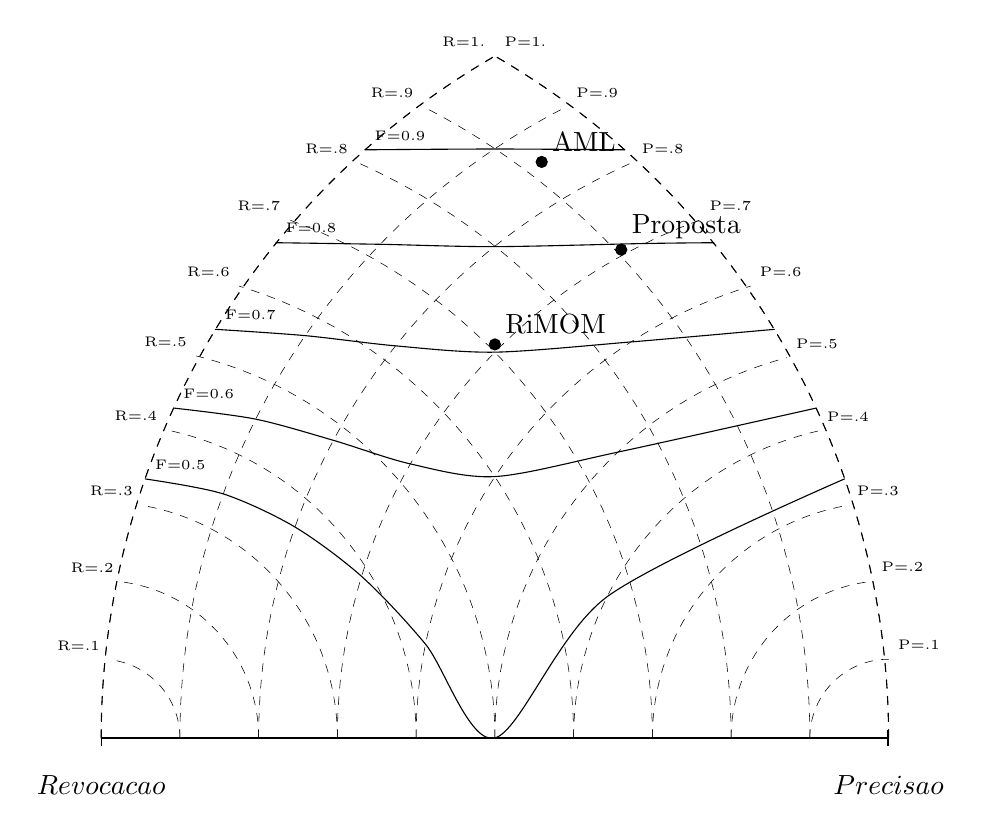
\begin{tikzpicture}[cap=round]{H}
		%\draw[step=1cm,very thin,color=gray] (0,0) grid (10.0,9.0);
		\draw[|-|] (-0,0) -- (10,0);
		\draw[dashed,very thin] (10,0) arc (0:60:10cm);
		\draw[dashed,very thin] (0,0) arc (180:120:10cm);
		\draw[dashed] (10,0) arc (0:60:10cm) node[anchor=south east]  {{\tiny R=1.}};
		\draw[dashed,very thin] (9,0) arc (0:63:9cm) node[anchor=south east] {{\tiny R=.9}};
		\draw[dashed,very thin] (8,0) arc (0:66:8cm) node[anchor=south east]  {{\tiny R=.8}};
		\draw[dashed,very thin] (7,0) arc (0:70:7cm) node[anchor=south east]  {{\tiny R=.7}};
		\draw[dashed,very thin] (6,0) arc (0:73:6cm) node[anchor=south east]  {{\tiny R=.6}};
		\draw[dashed,very thin] (5,0) arc (0:76:5cm) node[anchor=south east] {{\tiny R=.5}};
		\draw[dashed,very thin] (4,0) arc (0:78:4cm) node[anchor=south east] {{\tiny R=.4}};
		\draw[dashed,very thin] (3,0) arc (0:80:3cm) node[anchor=south east] {{\tiny R=.3}};
		\draw[dashed,very thin] (2,0) arc (0:82:2cm) node[anchor=south east] {{\tiny R=.2}};
		\draw[dashed,very thin] (1,0) arc (0:84:1cm) node[anchor=south east] {{\tiny R=.1}};
		\draw[dashed] (0,0) arc (180:120:10cm) node[anchor=south west] {{\tiny P=1.}};
		\draw[dashed,very thin] (1,0) arc (180:117:9cm) node[anchor=south west] {{\tiny P=.9}};
		\draw[dashed,very thin] (2,0) arc (180:114:8cm) node[anchor=south west] {{\tiny P=.8}};
		\draw[dashed,very thin] (3,0) arc (180:110:7cm) node[anchor=south west] {{\tiny P=.7}};
		\draw[dashed,very thin] (4,0) arc (180:107:6cm) node[anchor=south west] {{\tiny P=.6}};
		\draw[dashed,very thin] (5,0) arc (180:105:5cm) node[anchor=south west] {{\tiny P=.5}};
		\draw[dashed,very thin] (6,0) arc (180:103:4cm) node[anchor=south west] {{\tiny P=.4}};
		\draw[dashed,very thin] (7,0) arc (180:100:3cm) node[anchor=south west] {{\tiny P=.3}};
		\draw[dashed,very thin] (8,0) arc (180:96:2cm) node[anchor=south west] {{\tiny P=.2}};
		\draw[dashed,very thin] (9,0) arc (180:90:1cm) node[anchor=south west] {{\tiny P=.1}};
		\draw (0.56,3.29) node[anchor=south west] {\tiny{F=0.5}};
		\draw plot[smooth] coordinates { (0.56,3.29) (1.55,3.10) (2.46,2.68) (3.31,2.05) (4.12,1.19) (5.00,0.00) (6.42,1.79) (9.44,3.29)};
		\draw (0.92,4.19) node[anchor=south west] {\tiny{F=0.6}};
		\draw plot[smooth] coordinates { (0.92,4.19) (1.96,4.05) (2.95,3.78) (3.93,3.48) (5.00,3.32) (6.56,3.63) (9.08,4.19)};
		\draw (1.45,5.19) node[anchor=south west] {\tiny{F=0.7}};
		\draw plot[smooth] coordinates { (1.45,5.19) (2.59,5.11) (3.74,4.98) (5.00,4.90) (6.73,5.03) (8.55,5.19)};
		\draw (2.22,6.29) node[anchor=south west] {\tiny{F=0.8}};
		\draw plot[smooth] coordinates { (2.22,6.29) (3.54,6.27) (5.00,6.24) (6.91,6.28) (7.78,6.29)};
		\draw (3.35,7.47) node[anchor=south west] {\tiny{F=0.9}};
		\draw plot[smooth] coordinates { (3.35,7.47) (5.00,7.48) (6.65,7.47)};
		\draw (0,-0.6) node {$Revocacao$};
		\draw (10,-0.6) node {$Precisao$};
		%\draw (-0.2,0) node {0}; 
		%\draw (10.2,0) node {1}; 
		\draw plot[mark=*,] coordinates {(6.604935,6.20148640616)};
		\draw (6.614935,6.21148640616) node[anchor=south west] {Proposta};
		\draw plot[mark=*,] coordinates {(5.0,4.99848977192)};
		\draw (5.01,5.00848977192) node[anchor=south west] {RiMOM};
		\draw plot[mark=*,] coordinates {(5.594625,7.31602836991)};
		\draw (5.604625,7.32602836991) node[anchor=south west] {AML};
		\end{tikzpicture}
		\caption{Resultado das ferramentas para o cenário 2}
		\label{fig:cenario2}
\end{figure}
\end{center}

%\subsection{Verificação das hipóteses}
A seguir serão apresentados os resultados mapeados para suas respectivas hipóteses. A primeira hipótese refere-se à precisão apresentada pelas ferramentas. As hipóteses nula e alternativa estão numeradas abaixo, respectivamente:

\begin{itemize}
\item \textbf{H1-0:} A precisão apresentada pelas abordagens é igual.
\item \textbf{H1-1:} A precisão apresentada pelas abordagens é diferente.
\end{itemize}

Para realizar a análise, devemos observar a precisão nos dois cenários de alinhamento. Como descrito na Tabela \ref{tab:resultados}, a proposta apresentou precisão de 1 para o cenário 1 e 0.906 para o cenário 2.

A próxima validação de hipótese se refere à revocação. As hipóteses nula e alternativa estão numeradas abaixo, respectivamente:

\begin{itemize}
\item \textbf{H2-0:} A revocação apresentada pelas abordagens é igual.
\item \textbf{H2-1:} A revocação apresentada pelas abordagens é diferente.
\end{itemize}

Diante do resultado apresentado pela proposta nos dois cenários de alinhamento, onde apresentou uma revocação de 0.875 para o cenário C1 e 0.707 para o cenário C2. Apesar do bom desempenho, a proposta apresentou valores iguais a pelo menos uma das ferramentas em cada um dos cenários.

Finalizando a verificação de hipóteses, são analisadas as hipóteses relacionadas à medida-f. As hipóteses nula e alternativa estão listadas abaixo, respectivamente:

\begin{itemize}
\item \textbf{H3-0:} A medida-f apresentada pelas abordagens é igual.
\item \textbf{H3-1:} A medida-f apresentada pelas abordagens é diferente.
\end{itemize}

Conforme os resultados apresentados na Tabela \ref{tab:resultados}, a proposta ficou em primeira posição no cenário 1 com uma medida-f de 0.933 e segunda posição no cenário 2 com 0.794.

Para a análise estatística inferencial, visando a validação das hipóteses, utilizamos o teste de Fisher \cite{fisher1922mathematical} para comparar os pares das métricas. Esse teste pode ser usado para analisar a significância estatística da amostra. Com isso, é possível aceitar ou refutar qualquer uma das hipóteses, entre outras palavras, verificar se os resultados obtidos possuem diferenças estatísticas. Para isso, usou-se os resultados obtidos no experimento como entrada, seguindo a configuração apresentada na Tabela \ref{tab:resultados}. Como resultado, o teste estatístico apresentou p-valor igual a 0.8333, indicando que as ferramentas apresentam eficácia similar em relação às métricas. Consequentemente, não é possível refutar nenhuma das hipóteses nulas.

\section{Principais conclusões}
O experimento conduzido neste capítulo, visou avaliar a eficácia das ferramentas de alinhamento de dados conectados com relação às métricas de precisão, revocação e medida-f. Essas variáveis foram avaliadas separadamente em cada um dos dois cenários C1 e C2. No cenário C1, os dados apresentam 9 tipos de heterogeneidade ( \textit{e.g.}, multilinguagem, diferença nos catálogos, diferença fonética, diferentes graus de descrição). No cenário C2, os dados apresentam conjuntos instâncias similares, havendo apenas uma correspondência possível, o que caracteriza as demais instâncias como falso-positivas.

Diante dos resultados apresentados pelo teste estatístico, tem-se que as ferramentas apresentam eficácia similar para ambos os cenários analisados.  Contudo, pelas análises realizadas sobre as métricas, foi possível verificar que a proposta se destacou apenas em um dos cenários, o C1. Entretanto, deve-se ressaltar que a bordagem proposta não utiliza implementações específicas para os \textit{datasets} analisados, permitindo que seja utilizada em outros contextos com facilidade.